
\documentclass{package/notes}
\usepackage[english]{babel}
\usepackage{amssymb,amsmath,amsfonts}  %%% for maths
%%%%%%%%%%%%%%%%%%%%%%%%%%%%%%%%%%%%%
\usepackage{package/color-env}
\usepackage{lipsum}
\usepackage{graphicx}
\renewcommand\qedsymbol{$\blacksquare$}
%%%%%%%%%%%%%%%%%%%%%%%%%%%%%%%%%%%%%

\begin{document}

	\begin{titlepage} % Suppresses headers and footers on the title page
		
		\centering % Centre everything on the title page
		
		\scshape % Use small caps for all text on the title page
		
		\vspace*{\baselineskip} % White space at the top of the page
		
		%------------------------------------------------
		%	Title
		%------------------------------------------------
		
		\rule{\textwidth}{1.6pt}\vspace*{-\baselineskip}\vspace*{2pt} % Thick horizontal rule
		\rule{\textwidth}{0.4pt} % Thin horizontal rule
		
		\vspace{0.75\baselineskip} % Whitespace above the title
		
		{\huge Multivariable Calculus\\} % Title
		
		\vspace{0.75\baselineskip} % Whitespace below the title
		
		\rule{\textwidth}{0.4pt}\vspace*{-\baselineskip}\vspace{3.2pt} % Thin horizontal rule
		\rule{\textwidth}{1.6pt} % Thick horizontal rule
		
		\vspace{2\baselineskip} % Whitespace after the title block
		
		%------------------------------------------------
		%	Subtitle
		%------------------------------------------------
		
		\LARGE{Public Notes for Any Multivariable Calculus Course} 
		
		\vspace*{3\baselineskip} % Whitespace under the subtitle
		
		
		
		\vspace{0.5\baselineskip} 
		
		\vspace{0.5\baselineskip} 
		
		
		\vfill 
		
		%------------------------------------------------
		% Author
		%------------------------------------------------
		
		
		\vspace{0.3\baselineskip} 
		
		
		{\large Edited by\\  Trevor Bushnell} 
		
	\end{titlepage}
	\tableofcontents
%\newpage
\chapter{Vectors and the Geometry of Space}

\section{3D Coordinate Systems}

\subsection{About 3D Coordinate Systems}

\begin{itemize}
	\item We are used to working in textbf{planes} (1D input and 1D output), and we can model each input and output on a 2D plane
	\item Multivariable calculus is all about representing points in \textbf{space} (2D input and 1D output)
	\item There are 2 \textit{axes} in 2D space $\to$ there are textbf{3 axes} in 3D space
	\item There are 4 \textit{quadrants} in 2D space $\to$ there are 8 \textbf{octants} in 3D space
	\item There is \textit{one plane} in 2D space ($xy$-plane) $\to$ there are \textbf{3 planes} in 3D space ($xy$-plane, $xz$-plane, and $yz$-plane)
	\item Points in 2D space have \textit{2 coordinates} $\to$ points in 3D space have \textbf{3 coordinates}
	\item We went from creating \textit{graphs} in 2D space to creating \textbf{surfaces} in 3D space
	\item If you have a hard time visualizing 3D space, use the room around you and pick a bottom corner in the room
	\begin{itemize}
		\item Floor is $xy$-plane
		\item Left wall is $xz$-plane
		\item Right wall is $yz$-plane
	\end{itemize}
\end{itemize}

\subsection{The Distance Formula (3D)}

\begin{itemize}
	\item Distance formula in 3D is very similar to the distance formula in 2D
	\item Finds the distance between point $P_1$ and $P_2$ 
\end{itemize}

\newpage
\begin{definition}[The 3D Distance Formula]{def:label}
	To find the distance between two points $P_1(x_1, y_1, z_1)$ and $P_2(x_2,y_2,z_2)$, use the following distance formula:
	$$D = \sqrt{(x_2-x_1)^2 + (y_2-y_1)^2 + (z_2-z_1)^2}$$
\end{definition}

\subsection{Equation of a Sphere}
	
We will be representing many surfaces and it is important to understand the different types of surfaces that we will encounter. A basic one is a sphere, which looks like the following:
	
\begin{proposition}[The Equation of a Sphere]{prop:label}
The equation of a sphere with center $C(h,k,l)$ and radius $r$ is
$$(x-h)^2 + (y-k)^2 + (r-l)^2 = r^2$$
\end{proposition}


\section{Vectors}

\subsection{About Vectors}

\begin{definition}[Vectors]{def:label}
	A \textbf{vector} is a quantity that has both a \textit{direction} and a \textit{magnitude} (length).\\

	Ex: 60mph North is a vector because it has a magnitude (60mph) and a direction (North)\\

	We denote a vector by using either boldface ($\mathbf v$) or drawing an arrow over the name of the vector ($\mathbf v$)
\end{definition}

\begin{itemize}
	\item $\mathbf{0}$ is called the "zero vector and has length $0$ and no direction
\end{itemize}

\subsection{Vector Components and Magnitudes}

\begin{itemize}
	\item A vector algebraically looks like this $\to \mathbf{a} = <a_1, a_2>$ 
	\begin{itemize}
		\item The coordinates of $\mathbf a$ are the \textbf{components} of
		$\mathbf a$ 
	\end{itemize}
	\item NOTE: Vectors in textbook are represented with boldfont ($\vec{v}$) whereas when handwritten they are expressed with arrows ($\mathbf{v}$) %MARKER
\end{itemize}

\newpage
\begin{proposition}[Vector Components]{prop:label}
	The algebraic representation of a vector between points $A(x_1, y_1, z_1)$ and\\ B$(x_2, y_2,z_2)$ is
	$$\mathbf a = <x_2-x_1,y_2-y_1,z_2-z_1>$$\\

	To find the x-component of a vector, you can use the formula:
	$$\mathbf a_x = ||\mathbf a||\cos\theta$$\\

	To find the y-component of a vector, you can use the formula:
	$$\mathbf a_x = ||\mathbf a||\cos\theta$$\\

	Where $\theta$ is the angle between the vector and the x-axis
\end{proposition}

\begin{proposition}[Magnitudes of Vectors]{prop:label}
	To find the magnitude of the vector $\mathbf a$, use the distance formula (2D in the case of working with vectors having 2 components, 3D in the case of working with vectors with 3 components):

	\begin{equation*}
		\begin{aligned}
			||\mathbf a|| =&\: \sqrt {a_1^2 + a_2^2 + a_3^2}\\
			&OR\\
			||\mathbf a|| =&\: \sqrt {a_1^2 + a_2^2}\\
		\end{aligned}
	\end{equation*}
\end{proposition}

\subsection{Adding Vectors}

\begin{itemize}
	\item TIP TO TAIL METHOD: Put the end of the second vector on the tip of the first vector \textit{without changing the direction of length}
	\begin{itemize}
		\item The vector connecting the tail of the first vector to the tip of the second vector is the sum of the two vectors
	\end{itemize}
	\item ALGEBRAICALLY: To add two vectors, add together their components
	\item To subtract two vectors, subtract their components
\end{itemize}

\subsection{Other Properties of Vectors}

\begin{itemize}
	\item To multiply a vector by a scalar (any number), multiply that scalar by each component of the vector
	\item Other properties of vectors can be found below: 
	
	\begin{figure*}[h]
		\begin{center}
			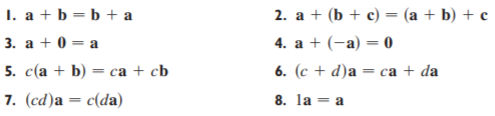
\includegraphics[width=10cm]{images/1.2.1_Image.PNG}
		\end{center}
	\end{figure*}
\end{itemize}

\subsection{Basis Vectors}

\begin{itemize}
	\item Vectors can also be written in relation to the unit vectors in the x, y, and z directions respectively (known as the \textbf{basis vectors})
	\item $\mathbf{i} = <1,0,0>$ is the \textbf{basis vector in the $x$-direction}
	\item $\mathbf{j} = <0,1,0>$ is the \textbf{basis vector in the $y$-direction}
	\item $\mathbf{k} = <0,0,1>$ is the \textbf{basis vector in the $z$-direction}
	\item To write up a vector $\mathbf a$ using components, you can add the components of $\mathbf a$ multiplied by the basis vectors
	\begin{itemize}
		\item Ex: $\mathbf a = a_x\mathbf i + a_y\mathbf j + a_z\mathbf k$
	\end{itemize}
\end{itemize}

\subsection{Applications}

\begin{itemize}
	\item Vectors can be used to represent motion (displacement, position, velocity, acceleration)
	\item Vectors are commonly used to describe \textbf{forces} because all forces are applied with a certain strength (magnitude measure in Newtons) and acting in a certain direction (expressed in angles)
\end{itemize}



\section{The Dot Product}

\subsection{Definition of the Dot Product}

\begin{definition}[The Dot Product]{def:label}
	If $\mathbf{a} = <a_1, a_2, a_3>$ and $\mathbf{b} = <b_1, b_2, b_3>$, then the \textbf{dot product of $\mathbf{a}$ and $\mathbf{b}$} is:

	$$\mathbf a \cdot \mathbf b = a_1b_1 + a_2b_2 + a_3b_3$$
\end{definition}

\begin{itemize}
	\item The result of a dot product is a \textit{scalar} and \textbf{not a vector}
	\item The dot product obeys many of the laws that hold true for ordinary products
\end{itemize}

\begin{proposition}[Physics Definition of the Dot Product]{prop:label}
	If $\theta$ is the angle between the vectors $\mathbf a$ and $\mathbf b$, then $ \mathbf a \cdot \mathbf b = |\mathbf a|\:|\mathbf b |\cos\theta$
\end{proposition}


\subsection{What Does the Dot Product Represent?}

\begin{itemize}
	\item Measures the angle between two vectors
\end{itemize}

\begin{proposition}[Angle Bweteen Two Vectors]{def:prop}
	The angle between two vectors can be found using the following formula:
	$$\theta = \cos ^{-1}\left(\frac{\mathbf a \cdot \mathbf b}{|\mathbf a | |\mathbf b|}\right)$$
	Where $\theta$ is the angle between vectors $\mathbf{a}$ and $\mathbf{b}$
\end{proposition}

\begin{itemize}
	\item Two vectors are \textit{orthogonal} if and only if $\mathbf a \cdot \mathbf b = 0$ 
	\item Dot products also help model the scalar projection of one vector onto another variable
	\end{itemize}

\begin{proposition}[Scalar Projections]{prop:label}
	Scalar projection of $\mathbf b$ onto $\mathbf a$: $\text{comp}_a b = \frac{\mathbf a \cdot \mathbf b}{|\mathbf a|}$ \\
	Vector projection of $\mathbf b$ onto $\mathbf a$: $\text{proj}_{\mathbf a}\mathbf b = \frac{\mathbf a \cdot \mathbf b}{|\mathbf a|^2}\mathbf a$
\end{proposition} % Clarify on what this means a little bit more and make sure that I have the terminology correct


\subsection{Direction Angles and Direction Cosines}

\begin{itemize}
	\item \textbf{DIRECTION ANGLES:} The angles $\alpha, \beta, \gamma$ in the interval $[0,\pi]$ that a vector makes with the positive x, y, or z axes respectively
	\item \textbf{DIRECTION COSINES:} The cosines of the direction angles
\end{itemize}

\begin{proposition}[Direction Cosines]{prop:label}
	$$
	\begin{aligned}
		\cos \alpha =& \frac{a_x}{|\mathbf{a}|}\\
		\cos \beta =& \frac{a_y}{|\mathbf a|}\\
		\cos \gamma =& \frac{a_z}{|\mathbf a|}
	\end{aligned}
	$$
\end{proposition}

\begin{itemize}
	\item The direction cosines of $\vec a$ are the components of the unit vector in the direction of $\vec a$ 
\end{itemize}

\begin{proposition}[Using Direction Cosines to Compute the Unit Vector]{prop:label}
	$$\frac{1}{|\vec a|}\vec a = <\cos\alpha, \cos\beta, \cos\gamma>$$
\end{proposition}

\section{The Cross Product}

\subsection{Definition of the Cross Product}

\begin{itemize}
	\item The cross product is another way to multiply vectors
	\item As opposed to a dot product, the cross product returns \textbf{a new vector that is orthogonal to the vectors being crossed}
\end{itemize}

\begin{definition}[The Cross Product]{def:label}
	If $\vec a = <a_1,a_2,a_3>$ and $\vec b = <b_1,b_2,b_3>$, then the **cross product of** $\vec a$ and $\vec b$ is:

	$$\vec a \times \vec b = <a_2b_3 - a_3b_2, a_3b_1-a_1b_3, a_1b_2 - a_2b_1>$$

	Instead of memorizing this, an easier way to remember how to compute the cross product is to put the two vectors you wish to cross into a matrix along with the basis vectors and compute the determinant of the 3 x 3 matrix.

	$$
	\vec a \times \vec b = \text{det}\left(\left[
	\begin{array}{ccc}
		\mathbf i & \mathbf j & \mathbf k\\
		a_1 & a_2 & a_3 \\
		b_1 & b_2 & b_3 \\
	\end{array}
	\right]\right)
	$$
\end{definition}

\begin{proposition}[Alternate Interpretation of the Cross Product]{prop:label}
	If $\theta$ is the angle between $\vec a$ and $\vec b$ and $0\le\theta\le\pi$, then:
	$$|\vec a \times \vec b | = |\vec a||\vec b| \sin\theta$$
\end{proposition}

\begin{itemize}
	\item The cross product is NOT communicative (order matters)
	\item The cross product is NOT associative (parentheses matters)
	\item However, many of the other usual laws of algebra *do* hold for cross products
\end{itemize}

\subsection{What Does the Cross Product Represent?}

\begin{itemize}
	\item The magnitude of the cross product of two vectors is the area of the parallelogram that spans between the two vectors being crossed
	\item You can use the right-hand rule to determine the direction of the resultant vector
	\begin{itemize}
		\item If you point your index finger away from you and your middle finger to the left, your thumb  naturally points upward which is the direction of the cross product
	\end{itemize}
	\item Two vectors are parallel if and only if $\vec a \times \vec b = \vec 0$ 
\end{itemize}

\subsection{Scalar Triple Products}

\begin{itemize}
	\item \textbf{SCALAR TRIPLE PRODUCT:} The product $\vec a \cdot (\vec b \times \vec c)$ 
	\item \textit{VISUALIZATION:} If considering the parallelepiped determined by the span of vectors $\vec a, \vec b, \vec c$, then the magnitude of the scalar triple product is the volume of the parallelepiped
	\begin{itemize}
		\item In symbols: $V = |\vec a \cdot (\vec b \times \vec c)|$
		\item The visualization makes sense because the area of the base is a parallelogram (meaning the area is the magnitude of the cross product of $\vec c$ and $\vec b$) and $\therefore$ the height is equal to $h = |\vec a| |\cos \theta|$ so dot product (need $|\cos\theta|$ because what is $\theta>\frac{\pi}{2}$)
		\item If $ V = 0$, then the three vectors are \textbf{coplanar} (they all lie in the same plane)
	\end{itemize}
\end{itemize}

\subsection{Application: Torque}

\begin{itemize}
	\item \textbf{TORQUE:} The force exerted to produce a turning effect
\end{itemize}

\begin{definition}[Torque]{def:label}
	$$
	\begin{aligned}
		\tau = \vec r \times \vec F&\\
		|\tau| = |\vec r \times \vec F| = |\vec r|&|\vec F|\sin\theta
	\end{aligned}
	$$
\end{definition}


\section{Equations of Lines and Planes}

\subsection{Lines in 3D}

\begin{itemize}
	\item To determine a line in 2D, you need two points or a point and a slope
	\begin{itemize}
		\item To determine a line in 3D, you need a point and a direction (vector)
	\end{itemize}
\end{itemize}

\begin{definition}[Vector Equation for a Line]{def:label}
	$$\vec r = \vec r_0 + t\vec v$$

	Where $\vec r$ is the position vector of any arbitrary point on the line, $\vec r_0$ is the position vector of a point $P_0(x_0,y_0,z_0)$ on line $L$, $\vec v$ is a vector parallel to the line, and $t$ is a scalar.
\end{definition}

\begin{itemize}
	\item If the vector $\vec v$ is written in component form, we can rewrite the vector equation for a line as a set of parametric equations for the line $L$ 
\end{itemize}

\newpage
\begin{definition}[Parametric Equations for a Line]{def:label}
	You can express each component of a line int terms of a common variable (usually defined as $t$). This creates a system of equations all in terms of $t$ that express a given line.

	$$
	\begin{aligned}
		x =& x_0 + at\\
		y =& y_0+bt\\
		z =& z_0+ct
	\end{aligned}
	$$
\end{definition} % I need to clarify what each of the variables mean in this definition

\begin{definition}[Symmetric Equations for a Line]{def:label}
	These are a set of equations that eliminate the parameter in the parametric equations.

	$$
	\frac{x-x_0}{a}=\frac{y-y_0}{b}=\frac{z-z_0}{c}
	$$

	If one of the parameters $a,b,c = 0$, then we can still write symmetric equations but then we also know in what plane the line lies in. (Ex: if $a= 0$, then the line lies in the plane $x=x_0$)
\end{definition} % I need to clarify what each of the variables mean in this definition

\begin{definition}[Line Segments]{def:label}
	The line segment from $\vec r_0$ to $\vec r_1$ is given by the vector equation:

	$$\vec r(t) = (r-t)\vec r_0 + t\vec r_1$$

	Where $t$ lies on the interval from $[0,1]$.
\end{definition} % Need to go back and review myself wth the standard r means, maybe make a clarification on that

\subsection{Planes}

\begin{itemize}
	\item A plane in space is determined by a point $P_0(x_0,y_0,z_0)$ in the plane and a vector $\vec n$ that is orthogonal to the plane
\end{itemize}

\begin{definition}[Vector Equation of a Plane]{def:label}
	$$
	\vec n \cdot \vec r = \vec n \cdot \vec r_0\\
	OR\\
	\vec n \cdot (\vec r - \vec r_0) = 0
	$$
\end{definition} %Clarify what each of the variables mean

\begin{definition}[Scalar Equation of the Plane Through Point $P_0$ With Normal Vector $\vec{n}$]{def:label}
	If $\vec n = <a,b,c>$ and $\vec r = <x,y,z>$ and $\vec r_0 = <x_0,y_0,z_0>$, then the equation  of a plane is:

	$$a(x-x_0) +b(y-y_0)+c(z-z_0) = 0$$
\end{definition}

\begin{definition}[Linear Equation of a Plane]{def:label}
	$$ax +by+cz+d=0$$
\end{definition}

\begin{itemize}
	\item If you have two vectors that lie in the plane, you can take the cross product of those to vectors to find the normal vector of the plane (since the resulting vector from the cross product is orthogonal to 	the vectors being crossed)
	\item The formula for the distance between a point and a plane in the form $ax+by+cz+d=0$ is 
	$$
	D = \frac{|ax_1+by_1+cz_1+d|}{\sqrt{a^2+b^2+c^2}}
	$$
\end{itemize}



\chapter{Partial Derivatives}

\section{Functions of Several Variables}

\subsection{Functions of Two Variables}

\begin{itemize}
	\item A \textbf{function $f$ of two variables} is a rule that assigns to each ordered pair of real numbers $(x,y)$ in a set $D$ a unique real number denoted by $f(x,y)$
	\item $x$ and $y$ are independent variables
	\item $z$ is the dependent variable
	\item To find the value of $f(x,y)$, substitute the respective values of $x$ and $y$ given in the coordinates $(x,y)$
\end{itemize}

\subsection{Graphs}

\begin{itemize}
	\item If $f$ is a function of two variables with domain $D$, then the \textbf{graph} of $f$ is the set of all points $(x,y,z)$ in $R^3$ such that $z=f(x,y)$ and $(x,y) \in D$.
	\item While a graph in $R^2$ is a curve/line, a graph in $R^3$ is a surface that floats in space above it's domain (which lies in the xy-plane)
	\item The function $f(x,y) = ax+by+c$ is considered a \textbf{linear function}
	\begin{itemize}
		\item The graph of a linear function has the equation $z = ax+by+c$ or $ax+by-z+c=0$
	\end{itemize}
	\item NOTE: An entire sphere cannot be represented by a single function of $x$ and $y$. You will need to use the positive and negative square root to differentiate between the upper hemisphere and the lower hemisphere
\end{itemize}

\subsection{Level Curves}

\begin{itemize}
	\item The \textbf{level curves} of a function $f$ of two variables are the curves with equations $f(x,y)=k$ where $k$ is a constant that is in the range of $f$
	\item SIMPLER DEFINITION: A level curve is the set of all points in the domain of $f$ where $f$ takes on a given value $k$
	\begin{itemize}
		\item Shows where the graph of $f$ has a height of $k$
	\end{itemize}
\end{itemize}

\subsection{Functions of Three or More Variables}

\begin{itemize}
	\item A \textbf{function of three variables} is a rule that assigns to each ordered triple $(x,y,z)$ in a domain $D \in R^3$ a unique real number denoted by $f(x,y,z)$
	\item \textbf{Level surfaces} are the surfaces where the function $f$ takes on a given value $k$
	\item To represent functions of more than three variables, you can represent them using vectors... but this reaches into the linear algebra world and outside the scope of this course
\end{itemize}



\section{Limits and Continuity}

\subsection{Limits of Multivariable Functions}

\begin{definition}[Limits of Multivarriable Functions]{def:label}
	Let $f$ be a function of two variables whose domain $D$ includes points arbitrarily close to $(a,b)$. Then the \textbf{limit of $f(x,y)$ as $(x,y)$ approaches $(a,b)$} is $L$.\newline

	Numerically speaking, 
	$$\lim_{(x,y)\to(a,b)}f(x,y)=L$$

	if for every number $\varepsilon > 0$ there is a corresponding number $\delta > 0$ such that

	$$\text{if } (x,y)\in D \:\:\&\:\: 0<\sqrt{(x-a)^2+(y-b)^2}<\delta \text{ then } |f(x,y)-L|<\varepsilon$$
\end{definition}

\begin{itemize}
	\item There are other notations that you can use for the limits of multivariable functions
		\begin{figure*}[h]
			\begin{center}
				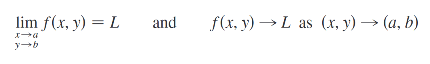
\includegraphics[width=12cm]{images/2.2.1_Image.PNG}
			\end{center}
		\end{figure*}
	\item $|f(x,y)-L|$ is the distance between the numbers $f(x,y)$ and $L$
	\item $\sqrt{(x-a)^2+(y-b)^2}$ is the distance between the point $(x,y)$ and $(a,b)$
	\item $\therefore$ the definition means that the distance between $f(x,y)$ and $L$ can be made arbitrarily small by making the distance between $(x,y)$ and $(a,b)$ arbitrarily small
	\item In the 2D calculus world, if the LHL didn't approach the same value as the RHL then the limit did not exist...
	\item ... however in 3D ($R^3$) there are an infinite number of directions from which you can approach $(a,b)$ so...

\begin{proposition}[Determining if a Limit Exists]
	If $f(x,y) \to L_1$ as $(x,y)\to (a,b)$ in one direction and $f(x,y) \to L_2$ as $(x,y)\to (a,b)$ in another direction and $L_1 \ne L_2$, then $\lim_{(x,y)\to(a,b)}f(x,y)$ \textbf{does not exist}
\end{proposition}

\begin{itemize}
	\item In order to show that a limit does not exist, you have to approach from multiple different directions
	\item Common directions to try:
	\begin{itemize}
		\item along the x-axis
		\item along the y-axis
		\item along the line $y=x$
		\item whatever hint the problem gives you (sometimes your professor/instructor will give you the directions to check to prove that a limit does or does not exist since infinitely many directions can make it daunting to find how a limit does not exist)
	\end{itemize}
	\item The \textbf{Limit Laws} from 2D Calculus still hold true in 3D
	\begin{itemize}
		\item The limit of a sum/difference/product/quotient is equal to the sum/difference/product/quotient of the limits
		\item The limit of a function times a constant is equal to that same constant times the limit of the function
	\end{itemize}
	\item The \textbf{Squeeze Theorem} still holds true from 2D Calculus
	\end{itemize}
\end{itemize}

\subsection{Continuity}

\begin{definition}[Continuity in 3D]{def:label}
	A function $f$ of two variables is called \textbf{continuous at $(a,b)$} if

	$$\lim_{(x,y)\to (a,b)} f(x,y) = (a,b)$$

	We say that $f$ is \textbf{continuous on D} if $f$ is continuous at every point $(a,b)$ in $D$.
\end{definition}

\begin{itemize}
	\item A function is continuous if the surface of a graph of a continuous function has no hole or break
	\item Using limit laws, the sum/difference/product/quotient of continuous functions are also continuous
\end{itemize}


\subsection{Functions of Three or More Variables}

$$\lim_{(x,y,z)\to (a,b,c)} = L$$

\begin{itemize}
	\item You can express limits of functions of three or more variables using vector notation, which is also outside the scope of the course
\end{itemize}



\section{Partial Derivatives}

\subsection{Definition of a Partial Derivatives}

\begin{definition}[Partial Derivatives]{def:label}
	The \textbf{partial derivative of $f$ with respect to $x$ at $(a,b)$} is:

	$$f_x(x,y) = \lim_{h\to 0} \frac{f(x+h,y)-f(x,y)}{h}$$

	The \textbf{partial derivative of $f$ with respect to $y$ at $(a,b)$} is:

	$$f_y(x,y) = \lim_{h\to 0} \frac{f(x,y+h)-f(x,y)}{h}$$
\end{definition}

\begin{itemize}
	\item If $z = f(x,y)$ then the notation for a partial derivative can be written as the following:
\end{itemize}

$$
\begin{aligned}
	f_x(x,y) =& f_x = \frac{\partial f}{\partial x} = \frac{\partial}{\partial x}f(x,y)=f_1=D_1f=D_xf\\
	f_y(x,y) =& f_y = \frac{\partial f}{\partial y} = \frac{\partial}{\partial y}f(x,y)=f_2=D_2f=D_yf\\
\end{aligned}
$$

\begin{proposition}[Rules for Partial Derivatives]{def:label}
	\begin{itemize}
		\item To find $f_x$, regard $y$ as a constant and differentiate $f(x,y)$ with respect to $x$.
		\item To find $f_y$, regard $x$ as constant and differentiate $f(x,y)$ with respect to $y$.
	\end{itemize}
\end{proposition}


\subsection{Interpretations of Partial Derivatives}

\begin{itemize}
	\item GEOMETRIC INTERPRETATION: Partial derivatives are the slopes of the tangent lines in the $x$ and $y$ directions to the point $(a,b)$ 
	\item partial derivatives can be interpreted as \textit{rates of change}
	\begin{itemize}
		\item $\frac{\partial z}{\partial x}$ represents the rate of change of z with respect to x when y is held constant
		\item $\frac{\partial z}{\partial y}$ represents the rate of change of z with respect to y when x is held constant
	\end{itemize}
\end{itemize}


\subsection{Functions of More Than Two Variables}

\begin{itemize}
	\item For any multivariable function, the number of partial derivatives is equal to the number of independent variables (one partial derivative for each independent variable)
	\item To find a partial derivative, simply hold every other independent variable constant
\end{itemize}


\subsection{Higher Order Derivatives}

\begin{itemize}
	\item Just like in 2D calculus when you can take the derivative over and over again to get a higher order derivative, you can do the same in 3D calculus
	\item However, when we take a higher order derivative, we have to specify with respect of what variable 
	\item the \textbf{second partial derivatives of $f$} are calculated in the following way:
\end{itemize}

$$
\begin{aligned}
	(f_x)_x=&f_{xx}=\frac{\partial}{\partial x}\left(\frac{\partial f}{\partial x}\right)=\frac{\partial^2f}{\partial x^2}=\frac{\partial^2 z}{\partial x^2}\\
	(f_x)_y=&f_{xy}=\frac{\partial}{\partial y}\left(\frac{\partial f}{\partial x}\right)=\frac{\partial^2f}{\partial y\partial x}=\frac{\partial^2 z}{\partial y \partial x}\\
	(f_y)_x=&f_{yx}=\frac{\partial}{\partial x}\left(\frac{\partial f}{\partial y}\right)=\frac{\partial^2f}{\partial x\partial y}=\frac{\partial^2 z}{\partial x \partial y}\\
	(f_y)_y=&f_{yy}=\frac{\partial}{\partial y}\left(\frac{\partial f}{\partial y}\right)=\frac{\partial^2f}{\partial y^2}=\frac{\partial^2 z}{\partial y^2}
\end{aligned}
$$

\begin{theorem}[Clairaut's Theorem]{theorem:label}
	Suppose $f$ is defined on a disk $D$ that contains the point $(a,b)$. If the functions $f_{xy}$ and $f_{yx}$ are both continuous on $D$, then:

	$$f_{xy}(a,b)=f_{yx}(a,b)$$
\end{theorem}

\subsection{Partial Differential Equations}

\begin{itemize}
	\item Partial differential equations are equations that contain partial derivatives and help express certain physical laws
	\item LAPLACE'S EQUATION: $$\frac{\partial^2u}{\partial x^2} + \frac{\partial^2u}{\partial y^2} = 0$$
	\begin{itemize}
		\item solutions of this equation are harmonic functions and help solve problems with heat conduction, fluid flow, electric potential
	\end{itemize}
	\item WAVE EQUATION: $$\frac{\partial^2u}{\partial t^2} = a^2\frac{\partial^2u}{\partial x^2}$$
	\begin{itemize}
		\item describes the motion of a waveform (ocean wave, sound wave, etc)
	\end{itemize}
\end{itemize}


\section{Tangent Planes and Linear Approximations}

\begin{itemize}
	\item In 2D calculus, we could approximate the value of a function using the tangent line
	\item In 3D calculus, we can approximate the value of a function using the tangent plane
\end{itemize}

\subsection{Tangent Planes}

\begin{itemize}
	\item \textbf{tangent plane:} the plane that is made up of the tangent lines in the x and y directions
\end{itemize}

\begin{definition}[Equation of a Tangent Plane]{def:label}
	Suppose $f$ has continuous partial derivatives. An equation of the tangent plane to the surface $z = f(x,y)$ at the point $P(a,b,c)$ is:

	$$z = f_x(a,b)(x-a)+f_y(a,b)(y-b)+c$$
\end{definition}

\begin{itemize}
	\item A multivariable function is \textit{differentiable} if the linear approximation is a good approximation when (x,y) is near (a,b)
\end{itemize}

\begin{proposition}[Defining Differentiability]{prop:label}
	If the partial derivatives $f_x$ and $f_y$ exist near $(a,b)$ and are continuous at $(a,b)$, then $f$ is differentiable at $(a,b)$
\end{proposition}


\subsection{Differentials}

\begin{itemize}
	\item In single variable calculus, we treat the differential $dx$ as an independent variable
	\item In multivariable calculus, we treat both $dx$ and $dy$ as indepentent variables
	\item $dz$ is called the \textit{total differential}
\end{itemize}

\begin{definition}[Differentials]{def:label}
	$$dz = f_x(x,y)dx+f_y(x,y)dy=\frac{\partial z}{\partial x}dx + \frac{\partial z}{\partial y}dy$$
\end{definition}

\begin{itemize}
	\item Based on the differential above, another way to write the linear approximation is: $$f(x,y) \approx f(a,b) + dz$$
\end{itemize}


\subsection{Functions of Three or More Variables}

\begin{itemize}
	\item Things are defined very similarly with more variables
	\item Linear Approximation: $$f(x,y,z) \approx f(a,b,c)+f_x(a,b,c)(x-a)+f_y(a,b,c)(y-b)+f_z(a,b,c)(z-c)$$
	\item Total Differential: $$dw = \frac{\partial w}{\partial x}dx + \frac{\partial w}{\partial y}dy + \frac{\partial w}{\partial z}dz$$
\end{itemize}



\section{The Chain Rule}

\subsection{Definition of the Chain Rule}

\begin{definition}[Chain Rule (Case I)]{def:label}
	If $z = f(x,y)$ is a differentiable function of $x$ and $y$ where $x = g(t)$ and $y = h(t)$ are both differentiable functions of $t$. Then $z$ is a differentiable function of $t$ and:

	$$\frac{dz}{dt}=\frac{\partial f}{\partial x}\frac{dx}{dt}+\frac{\partial f}{\partial y}\frac{dy}{dt}$$
\end{definition}

\begin{definition}[Chain Rule (Case II)]{def:label}
	If $z = f(x,y)$ is a differentiable function of $x$ and $y$, where $x = g(s,t)$ and $y = h(s,t)$ are differentiable functions of $s$ and $t$, then:

	$$
	\begin{aligned}
		\frac{\partial z}{\partial s}=&\frac{\partial z}{\partial x}\frac{\partial x}{\partial s}+\frac{\partial z}{\partial y}\frac{\partial y}{\partial s}\\
		\frac{\partial z}{\partial t}=&\frac{\partial z}{\partial x}\frac{\partial x}{\partial t}+\frac{\partial z}{\partial y}\frac{\partial y}{\partial t}	
	\end{aligned}
	$$
\end{definition}

\begin{itemize}
	\item If the independent variables are defined as single variable functions, then use \textbf{Case I} of the Chain Rule
	\item If the independent variables are defined as multi variable functions, then use \textbf{Case II} of the Chain Rule
\end{itemize}


\subsection{Implicit Differentiation}

\begin{itemize}
	\item The multivariable chain rule can be used to make implicit differentiation from single variable calculus significantly faster and easier:
\end{itemize}

\begin{proposition}[Implicit Differentiation with Multivariable Calculus (SV)]{prop:label}
	$$\frac{dy}{dx}=-\frac{\frac{\partial F}{\partial x}}{\frac{\partial F}{\partial y}}=-\frac{F_x}{F_y}$$
\end{proposition}

\begin{itemize}
	\item To derive Proposition 2.5.1, we assume that $F(x,y) = 0$ defines $y$ implicitly as a function of $x$
	\begin{itemize}
		\item Check the textbook \textit{Multivariable Calculus} by James Stewart to read why the assumption is valid (or check other textbooks or internet searches)
		% I should just copy what was said in the textbook 
	\end{itemize}
	\item We can similarly derive a different set of formulas to differentiate $\frac{\partial z}{\partial x}$ and $\frac{\partial z}{\partial y}$ 
\end{itemize}

\newpage
\begin{proposition}[Impliciit Definition with Multivariable Calculus (MV)]{prop:label}
	$$\frac{\partial z}{\partial x}=-\frac{\frac{\partial F}{\partial x}}{\frac{\partial F}{\partial z}}\:\:\:\:\:\:\:\:\:\:\:\:\:
	\frac{\partial z}{\partial y}=-\frac{\frac{\partial F}{\partial y}}{\frac{\partial F}{\partial z}}$$
\end{proposition}

\begin{itemize}
	\item Assumptions made: see text 
	% Copy from textbook into notes instead of making people look them up
\end{itemize}



\section{Directional Derivatives and the Gradient Vector}


\subsection{Directional Derivatives}

\begin{itemize}
	\item Partial derivatives can only find rates of change in the $x$ and $y$ directions
	\item If we want to find the rates of change in different directions, we must use the \textbf{directional derivative}
\end{itemize}

\begin{definition}[The Directional Dreivative]{def:label}
	The directional derivative in the direction of the \textit{unit}vector $\vec u = <a,b>$ is:

	$$D_uf(x_0,y_0)=\lim_{h\to 0}\frac{f(x_0+ha,y_0+hb)-f(x_0,y_0)}{h}$$
\end{definition}

\begin{theorem}[Computing a Directional Derivative]{theorem:label}
	$$D_uf(x,y) = f_x(x,y)a+f_y(x,y)b$$
\end{theorem}


\subsection{The Gradient Vector}

\begin{itemize}
	\item We can write the directional derivative as a dot product between a vector containing the partial derivatives and $\vec u$
	$$D_uf(x,y) = <f_x(x,y),f_y(x,y)> \cdot \:\vec u$$
	\item The vector containing the partial derivatives as components is called the \textbf{gradient vector}
	$$\nabla f(x,y) = <f_x(x,y),f_y(x,y)> \: =\frac{\partial f}{\partial x}\vec i+\frac{\partial f}{\partial y}\vec j$$
	\item Using the gradient notation, then the directional derivative becomes the following:
	$$D_uf(x,y) = \nabla f(x,y) \cdot \: \vec u$$
\end{itemize}


\subsection{Functions of Three or More Variables}

\begin{itemize}
	\item The directional derivative of $f$ at $(x_0, y_0, z_0)$ in the direction of the unit vector $\vec u = <a,b,c>$ is
	
	$$D_uf(x,y,z) = f_x(x,y,z)a + f_y(x,y,z)b + f_z(x,y,z)c$$

	\item the gradient vector is:
	$$\Delta f(x,y,z) = <f_x(x,y,z), f_y(x,y,z), f_z(x,y,z)$$

	\item this means that combined with the gradient vector, the directional derivative is:
	$$D_uf(x,y,z) = \Delta f(f,y,z) \cdot \mathbf{u}$$
\end{itemize}


\subsection{Maximizing the Directional Derivative}

\begin{itemize}
	\item Since there are infinitely many directional derivatives at any given point of $f$ (because we can go in infinitely many directions), we can ask ourselves in which direction does $f$ changes and what the value of this maximum rate of change is
\end{itemize}

\begin{theorem}[Maximizing the Directional Derivative]{theorem:label}
	Suppose $f$ is a differentiable function of two or three variables. The maximum value of the directional derivative $D_uf(\vec x)$ is $|\nabla f(\vec x)|$ and it occurs when $\vec u$ has the \textit{same direction as the gradient vector} $\nabla f(\vec x)$
\end{theorem}


\subsection{Tangent Planes to Level Surfaces}

\begin{itemize}
	\item The gradient vector at P is perpendicular to the tangent vector $\vec r'(t_0)$ to any curve C on S that passes through P
	\item $\therefore$ we can define the tangent plane to the level surface as the plane that passes though P and has normal vector $\nabla F(x_0,y_0,z_0)$ as the following:
	$$F_x(x_0,y_0,z_0)(x-x_0) + F_y(x_0,y_0,z_0)(y-y_0)+F_z(x_0,y_0,z_0)(z-z_0)=0$$
	\item the \textbf{normal line} to S at P is the line that passes through P while also being perpendicular to the tangent plane, $therefore$ the direction of the normal line is given by the gradien vector, meaning that the symmetric equations are as follows:
	$$\frac{x-x_0}{F_x(x_0,y_0,z_0)} = \frac{y-y_0}{F_y(x_0,y_0,z_0)}=\frac{z-z_0}{F_z(x_0,y_0,z_0)}$$
\end{itemize}


\subsection{Significance of the Gradient Vector}

\begin{itemize}
	\item Gradient vectors are perpendicular to level curves
	\item To draw a curve with the "steepest" change, draw a curve that is perpendicular to every level curve that it passes through
\end{itemize}



\section{Maximum and Minimum Values}

\begin{itemize}
	\item Just as we can use ordinary derivatives to find maximum and minimum values, we can use partial derivatives to find maximums and minimums of functions with two variables
\end{itemize}


\subsection{How to Find Local Maxima and Minima}

\begin{theorem}[The Partial Derivatives at a Local Max/Min]{theorem:label}
	If $f$ has a local maximum or minimum at $(a,b)$ and the first order partial derivatives of $f$ exist there, then $f_x(a,b) = 0$ and $f_y(a,b) = 0$ 
\end{theorem}

\begin{itemize}
	\item GEOMETRIC INTERPRETATION: if the graph of $f$ has a tangent plane at a local maximum or minimum, the tangent plane must be horizontal
	\item \textbf{critical point:} a point of $f$ where $f_x(a,b) = 0$ and $f_y(a,b) = 0$ or one of the partial derivatives does not exist
	\begin{itemize}
		\item Just like 2D calculus, \textit{not all critical points are maximums or minimums}
	\end{itemize}
\end{itemize}

\begin{proposition}[The Second Derivative Test]{prop:label}
	Suppose the second partial derivatives of $f$ are continuous on a disk with center $(a,b)$ and suppose that $(a,b)$ is a critical point of $f$.
	
	$$\text{Let } D =D(a,b)=f_{xx}(a,b)f_{yy}(a,b)-[f_{xy}(a,b)]^2$$

	\begin{itemize}
		\item If $D > 0$ and $f_{xx}(a,b) > 0$, then $f(a,b)$ is a local minimum
		\item If $D > 0$ and $f_{xx}(a,b) < 0$, then $f(a,b)$ is a local minimum
		\item If $D <0$, then $f(a,b)$ is a saddle point
	\end{itemize}
\end{proposition}

\begin{itemize}
	\item \textbf{saddle point:} a point that is neither a maximum nor a minimum
	\item If $D=0$ then the second derivative test \textbf{is inconclusive and gives no information}
	\item TIP: It can be helpful to remember D as a determinant: 
	$$D = \left[\begin{array}{cc}f_{xx}&f_{xy}\\f_{yx}&f_{yy}\end{array}\right] = f_{xx}f_{yy}-(f_{xy})^2$$
\end{itemize}


\subsection{Absolute Maximum and Minimum Values}

\begin{itemize}
	\item Just as a closed interval in 2D calculus contains the endpoints, a \textbf{closed set} in $R^2$ is one that contains all the boundary points
	\begin{itemize}
		\item Ex: $D = \{(x,y) | x^2+y^2\le1\}$ is a closed set because all the boundary points which are thee points that lie on the circle $x^2+y^2=1$ are contained in the set
	\end{itemize}
	\item \textbf{bounded set:} a set in $R^2$ that is contained within some disk ($\therefore$ it is finite to some extent)
\end{itemize}

\begin{theorem}[Extreme Value Theorem for Functions of Two Variables]{theorem:label}
	If $f$ is continuous on a closed, bounded set $D$ in $R^2$, then $f$ attains an absolute maximum value  and an absolute minimum value at some points in $D$. These points could be inside $D$ or could be one of the boundary points of $D$.
\end{theorem}

\begin{itemize}
	\item To find the absolute maximum and minimum values of a continuous function $f$ on a closed, bounded set $D$:
	\begin{enumerate}
		\item Find the values of $f$ at the critical points of $f$ in $D$
		\item Find the extreme values of $f$ on the boundary of $D$
		\item The largest of the values from the first two steps is the absolute maximum value and the smallest of the values from the first two steps is the absolute minimum value
	\end{enumerate}
\end{itemize}



\section{Lagrange Multipliers}


\subsection{Lagrange Multipliers with One Constraint}

\begin{itemize}
	\item Lagrange's method is a method that allows us to maximize/minimize a function subject to a constraint of the form $g(x,y,z) = k$
	\item Start by finding the extreme values of a function $f(x,y)$ that is restricted to lie on some level curve $g(x,y) = k$
	\item Find the largest value $c$ such that the level curve $f(x,y) = c$ intersects the level curve constraint $g(x,y) = k$
	\begin{itemize}
		\item This happens when the curves have a common tangent line, $\therefore$ the gradient vectors are parallel
	\end{itemize}
	\item \textbf{Lagrange Multiplier:} $\nabla f(x_0,y_0,z_0)=\lambda \nabla g(x_0,y_0,z_0)$
\end{itemize}

\begin{proposition}[Method of Lagrange Multipliers]{prop:label}
	To find the maximum and minimum values of $f(x,y,z)$ subject to the constraint $g(x,y,z) = k$ (assuming that the extreme values exist and that $\nabla g \ne \vec 0$ on the surface $g(x,y,z) = k$):

	\begin{enumerate}
		\item Find all the value of $x,y,z,\lambda$ such that
		$$
		\begin{aligned}
			\nabla f(x,y,z) &= \lambda \nabla g(x,y,z)\\
			&AND\\
			g(x,&y,z)=k
		\end{aligned}
		$$
		\item Evaluate $f$ at all the points $(x,y,z)$ that result from the first step. The largest of these values is the maximum value of $f$ and the smallest is the minimum value of $f$.
	\end{enumerate}
\end{proposition}

\begin{itemize}
	\item Expressing the equation from step 1 in terms of components results in the following equations:
	$$f_x = \lambda g_x\:\:\:\:f_y=\lambda g_y\:\:\:\:f_z=\lambda g_z\:\:\:\:g(x,y,z)=k$$
	\item For Lagrange Methods in two variables, we look for values $x,y,\lambda$ such that
	$$\begin{aligned}\nabla f(x,y) &= \lambda \nabla g(x,y)\\
	&AND\\g(x,&y) = k\end{aligned}$$
\end{itemize}

Which leads to solving three equations and a total of three unknowns:
$$f_x = \lambda g_x\:\:\:\:f_y=\lambda g_y\:\:\:\:g(x,y)=k$$


\subsection{Lagrange Multipliers with Two Constraints}

\begin{itemize}
	\item If we have two constraints, we look for a Lagrange Multiplier like this:
	$$\nabla f(x_0,y_0) = \lambda \nabla g(x_0,y_0) + \mu \nabla h(x_0,y_0)$$
	\item This results in solving the following system of equations:
	$$
	\begin{aligned}
		f_x=&\lambda g_x+\mu h_x\\
		f_y =& \lambda g_y + \mu h_y\\
		k =& g(x,y)\\
		c =& h(x,y)
	\end{aligned}
	$$
\end{itemize}

\chapter{Multiple Integrals}


\section{Double Integrals Over Rectangles}


\subsection{Review of Integrals}

\begin{itemize}
	\item With single integrals, we could split up the area into infinitely many rectangles with extremely small width to compute the area under a curve
	\item A single integral computes the \textit{area under a curve}
	\item We can approximate area under a curve using a Riemann Sum
\end{itemize}


\subsection{Volumes and Double Integrals}

\begin{itemize}
	\item A double integral computes the \textit{volume under a surface}
	\item If we define $f$ on a closed rectangle $R$ that has dimensions $[a,b]\times[c,d]$, then we can subdivide $R$ into an infinitely small number of rectangles and add up the volumes of the resulting (and really skinny) rectangular prisms
	\item We can approximate the volume under a surface using a Double Riemann Sum $$V \approx \sum_{i=1}^{m}\sum_{j=1}^{n} f(x_{ij}^*, y_{ij}^*)\Delta A$$
\end{itemize}

\begin{definition}[The Double Integral]{def:label}
	The \textbf{double integral} $f$ over the rectangle $R$ is:
	$$\iint_Rf(x,y)dA = \lim_{m,n\to\infty}\sum_{i=1}^{m}\sum_{j=1}^{n} f(x_{ij}^*, y_{ij}^*)\Delta A$$
\end{definition}

\begin{itemize}
	\item DOUBLE RIEMMAN SUM (w/ upper right corner rectangles): $\iint_Rf(x,y)dA = \lim_{m,n\to\infty}\sum_{i=1}^{m}\sum_{j=1}^{n} f(x_{i}, y_{j})\Delta A$
	\item If $f(x,y) \ge 0$, then the volume $V$ of the solid that lies above the rectangle $R$ and below the surface $z=f(x,y)$ is $V = \iint_R f(x,y) dA$ 
	\item \textbf{MIDPOINT RULE:} $\iint_Rf(x,y)dA \approx \sum_{i=1}^{m}\sum_{j=1}^{n} f(\bar{x_i},\bar{y_j})\Delta A$
	\begin{itemize}
		\item More accurate approximation for the volume under a surface
	\end{itemize}
\end{itemize}


\subsection{Average Value}

\begin{proposition}[The Average Value of a Function]{prop:label}
	The average value of a function of two variables defined on a rectangle $R$ is:

	$$f_{avg}=\frac{1}{A(R)}\iint_Rf(x,y)d$$

	where $A(R)$ is equal to the area of $R$.
\end{proposition}


\subsection{Properties of Double Integrals}

\begin{itemize}
	\item The double integral of a sum is the same as the sum of the double integrals
	\item The double integral of a constant times a function is equal to that constant times the double integral of the function
	\item If $f \ge g$ then the double integral of $f$ is $\ge$ the double integral of $g$
\end{itemize}




\section{Iterated Integrals}


\subsection{Definition of an Iterated Integral}

\begin{itemize}
	\item An \textbf{iterated integral} is the following: $\int_{a}^{b}\int_c^df(x,y)\:dy\:dx$
	\begin{itemize}
		\item We integrate with respect to y on the interval [c,d], then integrate what is left over with respect to x on the interval [a,b]
	\end{itemize}
	\item You can integrate in any order (wrt y or wrt x)- just make sure that you don't accidentally integrate x over y's interval on accident if you flip around!
	\item When solving iterated integrals, we work \textit{from the inside out}
\end{itemize}

\begin{theorem}[Fubini's Theorem]{theorem:label}
	If $f$ is continuous on the rectangle $R$ with dimensions $[a,b]\times[c,d]$, then:

	$$\iint_Rf(x,y)\:dA=\int_a^b\int_c^df(x,y)\:dy\:dx=\int_c^d\int_a^bf(x,y)\:dx\:dy$$

	More generally, this theorem is true if it is assumed that $f$ is bounded on $R$, $f$ is discontinuous only on a finite number of smooth curves, and the iterated integrals exist
\end{theorem}

\begin{itemize}
	\item You can also represent a double integral as a product of single integrals:
	$$\iint_R g(x)\:h(y)\:dA=\int_a^bg(x)\:dx\int_c^dh(y)\:dy\:\:\:\:\:R=[a,b]\times[c,d]$$
\end{itemize}



\section{Double Integrals Over General Regions}

\subsection{The Double Integral Dilemma}

\begin{itemize}
	\item When computing single integrals, we are always computing over an interval
	\item With double integrals, we don't always want to compute integrals over rectangles, but rather over general regions of weird and interesting shapes
	\item $\iint_Df(x,y)\:dA=\iint_RF(x,y)\:dA$ where $F(x,y) = \begin{cases}f(x,y); (x,y)\in D\\0;(x,y)\in R \:\&(x,y)\notin D\end{cases}$
	\item \textbf{Type I Region:} a domain that lies between the graphs of two continuous functions of x
	\item \textbf{Type II Regions:} a domain that lies between the graphs of two continuous functions of y
\end{itemize}

\begin{proposition}[Evalutaing the Double Integral Over a Type I Region]{prop:label}
	If $f$ is continuous on a type I region $D$, then:

	$$\iint_Df(x,y)\:dA=\int_a^b\int_{g_1(x)}^{g_2(x)}f(x,y)\:dy\:dx$$
\end{proposition}

\begin{proposition}[Evaluating the Double Integral Over a Type II Region]{prop:label}
	If $f$ is continuous on a type II region $D$, then:

	$$\iint_Df(x,y)\:dA=\int_c^d\int_{h_1(y)}^{h_2(y)}f(x,y)\:dx\:dy$$
\end{proposition}

\begin{itemize}
	\item TIP: Drawing a diagram of $D$ can help you figure out over what region you are integrating
	\item Draw errors to see how you integrate over the region
	\begin{itemize}
		\item Type I Region: arrow from bottom to top
		\item Type 2 Region: arrow from left to right
	\end{itemize}
\end{itemize}


\subsection{Properties of Double Integrals}

\begin{itemize}
	\item All of the double integral properties from 3.2 also hold up here as well
	\item You can split up a double integral into two double integrals over the split region
	$$\iint_Df(x,y)\:dA=\iint_{D_1}f(x,y)\:dA_+\iint_{D_2}f(x,y)\:dA$$
	\begin{itemize}
		\item In other words: if you can split up a region $D$ into two smaller regions, then you can take the double integral of $f$ wrt the different regions and add the result together
	\end{itemize}
	\item $\iint_D 1\:dA=A(D)$
	\item If $m\le f(x,y)\le M\: \forall \:(x,y) \in D$, then $mA(D) \le \iint_Df(x,y)\:dA\le MA(D)$
\end{itemize}



\section{Double Integrals in Polar Coordinates}


\subsection{Review of Polar Coordinates}

\begin{proposition}[Converting to Polar Coordinates]{prop:label}
	To convert from rectangular coordinates to polar coordinates (and vice-versa), use the following equations:

	$$
	\begin{aligned}
		x =& r\cos\theta\\
		y=&r\sin\theta\\
		r^2=&x^2+y^2\\
		\theta =& \tan^{-1}\left(\frac{y}{x}\right)	
	\end{aligned}
	$$
\end{proposition}


\subsection{Computing Double Integrals in Polar Coordinates}

\begin{definition}[A Double Integral in Polar Coordinates (Rectangular Region)]{def:label}
	If $f$ is a continuous function on a polar rectangle $R$ given by $0\le a\le r\le b$ and $\alpha\le\theta\le\beta$ where $0\le\beta-\alpha\le2\pi$, then

	$$\iint_Rf(x,y)\:dA=\int_\alpha^\beta\int_a^bf(r\cos\theta, r\sin\theta)r\:dr\:d\theta$$
\end{definition}

\begin{itemize}
	\item \textbf{WARNING: Be careful not to forget the additional factor of $r$ when computing a double integral in polar coordinates}
\end{itemize}

\begin{definition}[Computing Double Integrals in Polar Coordinates (General Region)]{prop:label}
	If $f$ is continuous over a general polar region, then:

	$$\iint_Df(x,y)\:dA =\int_\alpha^\beta\int_{h_1(\theta)}^{h_2(\theta)}f(r\cos\theta, r\sin\theta)r\:dr\:d\theta$$
\end{definition}



\section{Applications of Double Integrals}


\subsection{Density and Mass}

\begin{itemize}
	\item mass is equal to the integral of a density function $$m = \iint_D\rho(x,y)\:dA$$
	\item the total charge is the integral of the charge density function $$Q=\iint_D\sigma(x,y)\:dA$$
\end{itemize}


\subsection{Moments and Centers of Mass}

\begin{itemize}
	\item \textbf{Moment of the entire lamina about the a-axis:} $\iint_Dy\:\rho(x,y)\:dA$
	\item \textbf{Moment of the entire lamina about the y-axis:} $\iint_D x\:\rho(x,y)\:dA$
	\item \textbf{Coordinates of the center of mass of a lamina} is:
	$$
	\begin{aligned}
		\bar{x} = \frac{M_y}{m}=&\frac{1}{m}\iint_Dx\:\rho(x,y)\:dA\\
		\bar{y} = \frac{M_y}{m}=&\frac{1}{m}\iint_dy\:\rho(x,y)\:dA\\
		\text{where } m=&\iint_D\rho(x,y)\:dA
	\end{aligned}
	$$
\end{itemize}

\subsection{Moments of Inertia}

\begin{itemize}
	\item \textbf{Moment of inertia about the x-axis:} $I_x=\iint_Dy^2\rho(x,y)dA$
	\item \textbf{Moment of inertia about the y-axis:} $I_y = \iint_Dx^2\rho(x,y)\:dA$
	\item \textbf{Moment of inertia about the origin:} $I_0=\iint_D(x^2+y^2)\rho(x,y)dA$
	\item $I_0=I_x+I_y$
	\item \textbf{radius of gyration of a lamina about an axis} is a number $R$ such that $mR^2 = I$
	\item \textbf{radius of gyration wrt x-axis:} $m\bar{\bar{y}}^2=I_x$ 
	\item \textbf{radius of gyration wrt y-axis:} $m\bar{\bar{x}}^2=I_y$
\end{itemize}


\subsection{Probability}

\begin{itemize}
	\item \textbf{joint density function of X and Y:} $P((X,Y)\in D)=\iint_Df(x,y)dA$
	\item $P(a\le X \le b, c \le Y \le d) = \int_a^b\int_c^df(x,y)\:dy\:dx$
	\item The joint density function has the following properties (because probabilities can't be negative and are measured on a scale from $0$ to $1$):
	$$
	\begin{aligned}
		f(x,y)\ge 0\;\;\;\;\;\;\;\;\;\;\;\;\iint_{R^2}f(x,y)\:dA = 1\\
		\iint_{R^2}f(x,y)\:dA=\int_{-\infty}^{\infty}f(x,y)\:dx\:dy=1
	\end{aligned}
	$$
\end{itemize}


\subsection{Expected Values}

\begin{itemize}
	\item \textbf{expected value} is a \textit{synonym for mean} and is represented in statistics by $\mu$
	\item $\mu_x=\iint_{R^2}xf(x,y)\:dA\;\;\;\;\;\;\;\mu_y=\iint_{R^2}yf(x,y)dA$
	\item \textbf{Normal distribution:} $f(x) = \frac{1}{\sigma\sqrt{2\pi}}e^{-\frac{(x-\mu)^2}{2\sigma^2}}$
\end{itemize}



\section{Triple Integrals}


\subsection{Definition of the Triple Integral}

\begin{definition}[The Triple Integral]{def:label}
	The \textbf{triple integral} of $f$ over box $B$ is:

	$$\iiint_Bf(x,y,z)\:dV=\lim_{l,m,n\to\infty}\sum_{i=1}^l\sum_{j=1}^{m}\sum_{k=1}^nf(x_{ijk}^*, y_{ijk}^*, z_{ijk}^*)\Delta V$$
\end{definition}

\begin{itemize}
	\item Fubini's Theorem also works for triple integrals (it doesn't matter the order that you integrate as long as you match the bounds to what you are integrating)
\end{itemize}

\begin{proposition}[Triple Integrals Over General Regions]{prop:label}
	The triple integral of $f$ over a general region $E$ is...\\

	\textit{Over a Type I region:}

	$$\iiint_Ef(x,y,z)dV=\int_a^b\int_{g_1(x)}^{g_2(x)}\int_{u_1(x,y)}^{u_2(x,y)}f(x,y,z)\:dz\:dy\:dx$$

	\textit{Over a Type II region:}

	$$\iiint_Ef(x,y,z)\:dV=\int_c^d\int_{h_1(y)}^{h_2(y)}\int_{u_1(x,y)}^{u_2(x,y)}f(x,y,z)\:dz\:dx\:dy$$
\end{proposition}


\subsection{Applications of the Triple Integral}

\begin{itemize}
	\item A triple integral is the volume of a solid that is "floating" somewhere in $R^3$
	\begin{itemize}
		\item Double integrals compute volumes of solids over regions, whereas with triple integrals each dimension of the solid is defined and is NOT just projected from a domain lying in a specific plane
	\end{itemize}
	\item \textbf{mass:} $m = \iiint_E \rho(x,y,z)\:dV$
	\item \textbf{moments:} $M_{yz}=\iiint_Ex\rho(x,y,z)\:dV\;\;\;M_{xz}=\iiint_Ey\rho(x,y,z)\:dV\;\;\;M_{xy}=\iiint_E z\rho(x,y,z)\:dV$
	\item \textbf{center of mass:} $\bar{x}=\frac{M_{yz}}{m}\;\;\;\bar{y}=\frac{M_{xz}}{m}\;\;\;\bar{z}=\frac{M_{xy}}{m}$
	\item \textbf{moments of inertia:} $I_x=\iiint_E(y^2+z^2)\rho(x,y,z)\:dV\;\;\;\;I_y=\iiint_E(x^2+z^2)\rho(x,y,z)\:dV\;\;\;\;I_z=\iiint_E(x^2+y^2)\rho(x,y,z)\:dV$
	\item \textbf{total electric charge:} $Q = \iiint_E \sigma(x,y,z)\:dV$
	\item \textbf{joint density function of X, Y, and Z:} $P((X,Y,Z)\in E)=\iiint_Ef(x,y,z)\:dV$
	\begin{itemize}
		\item $P(a\le X\le b, c\le Y\le d, r\le Z\le s)=\int_a^b\int_c^d\int_r^sf(x,y,z)\:dz\:dy\:dx$
		\item joint density function satisfies $f(x,y,z)\ge 0$ and $\int_{-\infty}^\infty\int_{-\infty}^\infty\int_{-\infty}^\infty f(x,y,z)\:dz\:dy\:dx=1$
	\end{itemize}
\end{itemize}



\section{Triple Integrals in Cylindrical Coordinates}


\subsection{What Are Cylindrical Coordinates?}

\begin{itemize}
	\item Cylindrical coordinates are represented by the ordered triple $(r,\theta,z)$, where $r$ and $\theta$ are polar coordinates of the projection of $P$ onto the $xy$-plane to $P$
	\item $r$ is the radius of a circle in the $xy$-plane
	\item $\theta$ is the angle of rotation in the $xy$-plane
\end{itemize}

\begin{definition}[Converting to Cylindrical Coordinates]{def:label} %make sure polar is def
	To convert from cylindrical coordinates to rectangular coordinates (and vice-versa), use the following equations:

	$$
	\begin{aligned}
		x =& r\cos\theta\\
		y=&r\cos\theta\\
		z=&z\\
		r^2 =& x^2 + y^2\\
		\theta =& \tan^{-1}\frac{y}{x}
		\end{aligned}
	$$
\end{definition}


\subsection{Evaluating Triple Integrals with Cylindrical Coordinates}

\begin{proposition}[Evaluating Triple Integrals in Cylindrical Coordinates]{prop:label}
	To evaluate a triple integral in cylindrical coordinates, use the following:

	$$\iiint_Ef(x,y,z)\:dV=\int_\alpha^\beta\int_{h_1(\theta)}^{h_2{\theta}}\int_{u_1(r\cos\theta)}^{u_2(r\cos\theta)}f(r\cos\theta,r\sin\theta,z)\:r\:dz\:dr\:d\theta$$
\end{proposition}

\begin{itemize}
	\item \textbf{WARNING: Don't forget to add in the extra factor of $r$ when converting from rectangular coordinates to spherical coordinates}
	\item Cylindrical coordinates make evaluating certain solids (such as cylinders) much easier to compute their integral
\end{itemize}



\section{Triple Integrals in Spherical Coordinates}


\subsection{What Are Spherical Coordinates?}

\begin{itemize}
	\item Spherical coordinates are represented by the ordered triple $(\rho,\theta,\phi)$
	\begin{itemize}
		\item $\rho$ is the radius
		\item $\theta$ is the angle of rotation in the $xy$-plane
		\item $\phi$ is the angle between the positive $z$-axis and $\rho$
	\end{itemize}
\end{itemize}

\begin{definition}[Converting to Spherical Coordinates]{def:label} %make sure this polar is def
	To convert between rectangular coordinates and spherical coordinates (and vice-versa), use the following formulas:

	$$
	\begin{aligned}
		x =&\rho\sin\phi\cos\theta\\
		y=&\rho\sin\phi\sin\theta\\
		z=&\rho\cos\phi\\
		\rho^2=&x^2+y^2+z^2
	\end{aligned}
	$$
\end{definition}

\begin{itemize}
	\item \textbf{WARNING:} There is not a universal agreement on the notation of spherical coordinates
	\begin{itemize}
		\item Some books reverse the meanings of $\theta$ and $\phi$ and use $r$ in place of $\rho$
	\end{itemize}
\end{itemize}


\subsection{Evaluating Triple Integrals With Spherical Coordinates}

\begin{proposition}[Evaluating Triple Integrals With Spherical Coordinates]{prop:label}
	To evaluate a triple integral in spherical coordinates, use the following formula:

	$$\iiint_Ef(x,y,z)\:dV=\int_c^d\int_\alpha^\beta\int_a^bf(\rho\sin\phi\cos\theta,\rho\sin\phi\sin\theta,\rho\cos\phi)\:\rho^2\sin\phi\:d\rho\:d\theta\:d\phi$$

	Where $E$ is a spherical wedge given by:

	$$E = \{(\rho,\theta,\phi)|a\le\rho\le b, \alpha\le\theta\le\beta,c\le\phi\le d\}$$
\end{proposition}

\begin{itemize}
	\item Triple integral over a general region: 
	
	$$\iiint_Ef(x,y,z)\:dV=\int_c^d\int_{h_1(\phi)}^{h_2(\phi)}\int_{u_1(\theta\phi)}^{u_2(\theta,\phi)}f(\rho\sin\phi\cos\theta,\rho\sin\phi\sin\theta,\rho\cos\phi)\:\rho^2\sin\phi\:d\rho\:d\theta\:d\phi$$

	\item \textbf{WARNING: Don't forget to add in the factor $\rho^2\sin\phi$ when converting from rectangular to spherical coordinates}
	\item Triple integrals make evaluating integrals with cones or spheres as their boundary significantly easier
\end{itemize}




\section{Change of Variables in Multiple Integrals}


\subsection{Taking What We Know and Extending to Generality}

\begin{itemize}
	\item We've already tried changing variables before!
	\item In 2D calculus, we would substitute $x$ for $u$ using the Substitution Rule
	\item In 3D calculus, we would substitute $x$ and $y$ using the polar coordinates conversion equations
	\item In this section, we learn a general way to change variables that is given by a \textbf{linear transformation $T$} from the $uv$-plane to the $xy$-plane: $T(u,v) = (x,y)$
	\begin{itemize}
		\item This is a linear algebra question at its heart
	\end{itemize}
	\item $x$ and $y$ are related by the equations $x = g(u,v)$ and $y=h(u,v)$
	\item We usually assume that $T$ is a $C^1$ transformation, which means that $g$ and $h$ have continuous first-order partial derivatives
	\item A linear transformation $T$ is just a function whose domain and range are both subsets of $R^2$
	\item If $T(u_1,v_1) = (x_1,y_1)$, then the point $(x_1,y_1)$ is in the \textbf{range} of $T$
	\item If no two points have the same associated range point, then $T$ is \textbf{one-to-one}
	\item If $T$ is a one-to-one transformation, then the \textbf{inverse transformation $T^{-1}$} from the $xy$-plane
	\item to the $uv$-plane can possibly be solved using the equations $u=G(x,y)$ and $v=H(x,y)$
\end{itemize}


\subsection{The Jacobian}

\begin{definition}[The Jacobian]{def:label}
	The \textbf{Jacobian} of the transformation $T$ given by $x=g(u,v)$ and $y=h(u,v)$ is:

	$$\frac{\partial(x,y)}{\partial(u,v)}=
	\left[
	\begin{array}{cc}
	\frac{\partial x}{\partial u}&\frac{\partial x}{\partial v}\\
	\frac{\partial y}{\partial u} & \frac{\partial y}{\partial v}
	\end{array}
	\right]$$

	Using this notation, we can approximate $\Delta A$ with:

	$$\Delta A \approx \left|\frac{\partial(x,y)}{\partial(u,v)}\right|\Delta u\:\Delta v$$
\end{definition}

\begin{proposition}[Change of Variables in a Jacobian]
	Suppose that T is a $C^1$ transformation whose Jacobian is nonzero and that maps a region $S$ into the $uv$-plane onto a region $R$ in the $xy$-plane. If $F$ is continuous on $R$ and that $R$ and $S$ are type I or type II plane regions AND that T is one-to-one, except perhaps on the boundary of $S$, then:

	$$\iint_R f(x,y)\:dA = \iint_Sf(x(u,v),y(u,v))\left|\frac{\partial(x,y)}{\partial(u,v)}\right|\Delta u\:\Delta v$$
\end{proposition}


\subsection{The Jacobian and Triple Integrals}

\begin{itemize}
	\item The Jacobian in $R^3$ is the following determinant:
	$$\frac{\partial(x,y,z)}{\partial(u,v,w)} = \iiint_Sf(x(u,v,w),y(u,v,w),z(u,v,w))\left|\frac{\partial(x,y,z)}{\partial(u,v,w)}\right|\Delta u\:\Delta v\:\Delta w$$
\end{itemize}





\chapter{Vector Calculus}


\section{Vector Fields}


\subsection{About Vector Fields}

\begin{definition}[Vector Fields]{def:label}
	Let $D$ be a set in $R^n$ ($\therefore$ a plane region). A \textbf{vector field on $R^n$} is a function $\vec F$ that assigns to each point $(x_1,x_2,...,x_i)$ in $D$ a $n$-dimensional vector
\end{definition}

\begin{itemize}
	\item Each point in a vector field represents a vector in space that starts at the indicated point
	\item You can get a reasonable impression for $F$ by drawing a few of the vectors in the vector field (since it is impossible to draw a vector for the infinite number of points in $D$)
	\item Because $\vec F$ is a vector, we can express $F$ in it's components- except that in this case each component is an individual function itself
	
	$$
	\begin{aligned}
		\vec F(x,y)=P(x,y)\vec i + Q(x,y) \vec j+ &R(x,y)\vec k= \:<P(x,y),Q(x,y),R(x,y)>\\
		\vec F(x,y) =& P\vec i + Q\vec j + R\vec k
	\end{aligned}
	$$
\end{itemize}

\begin{itemize}
	\item $P$, $Q$, and $R$ are called \textit{scalar fields} to be distinguished from vector fields
	\item To sketch a vector field, simply sketch a few of the vectors that are created from the vector function $\vec F$
	\item Vector fields can be used to model gravitation, fluid flow, weather, electricity flow, and more
\end{itemize}


\subsection{Gradient Fields}

\begin{itemize}
	\item Because the gradient of $f$ is technically a vector whose components are functions (partial derivatives are functions), $\nabla f$ is technically a vector field and is called the \textbf{gradient vector field}
\end{itemize}


\subsection{Vector Field Vocabulary}

\begin{itemize}
	\item A vector field $\vec F$ is called a \textbf{conservative vector field} if it is the gradient of some scalar function
	\begin{itemize}
		\item if there exists a function $f$ such that $\nabla f = \vec F$, then $\vec F$ is a conservative vector field
		\begin{itemize}
			\item $f$ would be considered the \textit{potential function} for $\vec F$
		\end{itemize}
	\end{itemize}
	\item Not all vector fields are conservative, but conservative vector fields do arise often in the application of physics
	\begin{itemize}
		\item The gravitation vector field is a conservative vector field
	\end{itemize}
\end{itemize}



\section{Line Integrals}


\subsection{Definition of Line Integrals}

\begin{itemize}
	\item Line integrals are similar to single integrals except that rather than integrating over an interval, you integrate over a curve $C$ defined by the parametric equations:
	
	$$
	\begin{aligned}
		x=x(t)\;\;\;\;\;\;y=&y(t)\;\;\;\;\;\;a\le t\le b\\
		&OR\\
		\vec{r} = x(t)&\vec i + y(t)\vec j
	\end{aligned}
	$$
\end{itemize}

\begin{definition}[Line Integrals]{def:label}
	If $f$ is defined on a smooth curve $C$ using the parametric equations (see above), then the \textbf{line integral of $f$ along $C$} is:

	$$\int_Cf(x,y)\:ds = \lim_{n\to\infty}\sum_{i=1}^nf(x_i^*,y_i^*)\Delta s_i$$
\end{definition}

\begin{proposition}[Computing a Line Integral]{prop:label}
	To evaluate the line integral, use the following formula:

	$$\int_Cf(x,y)\:ds=\int_a^bf(x(t),y(t))\sqrt{\left(\frac{dx}{dt}\right)^2+\left(\frac{dy}{dt}\right)^2}\:dt$$
\end{proposition}


\subsection{Computing Line Integrals in Different Ways}

\begin{itemize}
	\item If $C$ is a \textit{piecewise-smooth curve} ()$C$ is a union of a finite number of smooth curves $C_1,C_2,\cdots,C_i$) where the initial point of $C_{i+1}$ is the final point of $C_i$, then:
	
	$$\int_Cf(x,y)\:ds = \int_{C_1}f(x,y)\:ds + \int_{C_2}f(x,y)\:ds+\cdots+\int_{C_i}f(x,y)\:ds$$

	\item The interpretation of a line integral is based on the interpretation of the function $f$
	\begin{itemize}
		\item Ex: if $f$ represents the density of a wire, then the mass of the wire is the line integral of the density function
	\end{itemize}
\end{itemize}

\begin{proposition}[Evaluating Line Integrals w.r.t Independent Variables]{prop:label}
	To evaluate the \textbf{line integral of $f$ along $C$ wrt x:}

	$$\int_Cf(x,y)dx=\int_a^bf(x(t),y(t))x'(t)dt\\$$

	To evaluate the \textbf{line integral of $f$ along $C$ wrt y:}

	$$\int_Cf(x,y)dy=\int_a^bf(x(t),y(t))y'(t)dt$$
\end{proposition}

\begin{itemize}
	\item It happens frequently that the line integrals wrt x and y occur together, therefore it is OK to abbreviate using the following:
	
	$$\int_CP(x,y)dx+\int_cQ(x,y)dy=\int_CP(x,y)dx+Q(x,y)dy$$

	Even though by strict mathematical rules the above statement isn't true

	\item The hardest part of computing a line integral is figuring out how to set up the line integral with the correct parametric representation
	\begin{itemize}
		\item Often helpful to parameterize a line segment that starts at $\vec r_0$ and ends at $\vec r_1$ $$\vec r(t)=(1-t)\vec r_0+t\vec r_1\;\;\;\;0\le t \le 1$$
	\end{itemize}
	\item parameterization is important because it determines the \textbf{orientation} of a curve $C$ with the positive direction corresponding to increasing values for $t$
\end{itemize}


\subsection{Line Integrals in Space}

\begin{proposition}[Computing Line Integrals in Space]{prop:label}
	If $C$ is a smooth curve defined parametrically or defined by a vector valued function, then:
	$$\int_Cf(x,y,z)\:ds=\int_a^bf(x(t),y(t),z(t))\sqrt{\left(\frac{dx}{dt}\right)^2+\left(\frac{dy}{dt}\right)^2+\left(\frac{dz}{dt}\right)^2}\:dt$$
\end{proposition}

\begin{itemize}
	\item line integrals in 2D and 3D can be expressed under the same vector notation:
	$$\int_a^bf(\vec r(t))|\vec r'(t)|\:dt$$
	\begin{itemize}
		\item using this notation, if you know what $\vec r(t)$ is, then you know how many dimensions the vector has and you know whether your line integral lives in the plane or whether your line integral lives in space
	\end{itemize}
	\item Fun fact: the special case of $f(x,y,z) = 1$ results in $\int_C|\vec r'(t)|dt = L$ which is the same as the formula for the length of a curve defined parametrically from single-variable calculus
	\item When evaluating line integrals in space, it is possible to write line integrals using the following:
	$$\int_CP(x,y,z)\:dx+Q(x,y,z)\:dy+R(x,y,z)\:dz$$
\end{itemize}


\subsection{Line Integrals Over Vector Fields}

\begin{definition}[Line Integrals Over Vector Fields]{def:label}
	If $\vec F$ is a continuous vector field defined on a smooth curve $C$ given by a vector function $\vec r(t), a \le t \le b$, then the \textbf{line integral of $\vec F$ along $C$} is:

	$$\int_C\vec F\cdot d\vec r = \int_a^b\vec F\vec r(t)) \cdot \vec r'(t)\:dt=\int_C\vec F \cdot \vec T \:ds$$
\end{definition}

\begin{itemize}
	\item NOTE: Even though $\int_C \vec F \cdot d\vec r= \int_C \vec F \cdot \vec T \: ds$ and integrals wrt arc length are unchanged when orientation is reversed, it is still true that $\int_{-C}\vec f \cdot d\vec r = -\int_C\vec F \cdot d\vec r$
	\begin{itemize}
		\item This is because the unit tangent vector $\vec T$ is replaced by its negative when $C$ is replaced by $-C$
		
		$$\int_C \vec F \cdot d\vec r = \int_C P\:dx + Q\:dy + R\:dz\:\:\:
		\text{where } \vec F = P\vec i + Q\vec j + R\vec k$$
	\end{itemize}
\end{itemize}



\section{The Fundamental Theorem for Line Integrals}


\subsection{Definition of the Fundamental Theorem for Line Integrals}

\begin{itemize}
	\item Just as there is a Fundamental Theorem of Calculus for single variable calculus, there is a Fundamental Theorem for Line Integrals which is the FToC applied to line integrals
\end{itemize}

\begin{theorem}[The Fundamental Theorem for Line Integrals]{theorem:label}
	If $C$ is a smooth curve given by the vector function $\vec r(t), a\le t\le b$ and $f$ is a differentiable  function of two or three variables whose gradient vector $\nabla f$ is continuous on $C$, then:

	$$\int_C\nabla f\cdot d\vec r = f(\vec r(b)) - f(\vec r(a))$$

	In other words: we can evaluate the line integral of a conservative vector field simply by knowing the value of $f$ at the endpoints of $C$.
\end{theorem}

\begin{itemize}
	\item The line integral of $\nabla f$ is the net change in $f$
\end{itemize}


\subsection{Independence of Path}

\begin{itemize}
	\item If $C_1$ and $C_2$ are two piecewise-smooth curves (called *paths*) that have the same initial point $A$ and terminal point $B$, then:
	$$\int_{C_1}\nabla f\cdot d\vec r = \int_{C_2}\nabla f\cdot d\vec r$$
	\item IN GENERAL: If $\vec F$ is a continuous vector field with domain $D$, we say that the line integral $\int_C \vec F \cdot d\vec r$ is \textbf{independent of path} if $\int_{C_1}\nabla f\cdot d\vec r = \int_{C_2}\nabla f\cdot d\vec r$ for any two paths $C_1$ and $C_2$
	\begin{itemize}
		\item $\therefore$ line integrals of conservative vector fields are independent of path
	\end{itemize}
	\item a curve is \textbf{closed} if its terminal point is the same as its initial point ($\vec r(b) = \vec r(a)$)
	\item a curve is \textbf{open} if for every point $P$ in $D$ there is a disk with center $P$ that lies entirely in $D$
	\item a domain $D$ is \textbf{connected} if any two points in $D$ can be joined by a path that lies in $D$
	\item a \textbf{simple curve} is a curve that doesn't intersect itself anywhere between its endpoints
\end{itemize}

\begin{theorem}[Line Integrals and Independence of Path]{theorem:label}
	$\int_C \vec F \cdot d\vec r$ is independent of path in $D$ if and only if $\int_C \vec F \cdot d\vec r = 0$ for every closed path $C$ in $D$
\end{theorem}

\begin{itemize}
	\item Work done by a conservative force field as it moves an object around a closed path is $0$
\end{itemize}

\begin{theorem}[Independent of Path Implies Conservatism]{theorem:label}
	If $\vec F$ is a vector field that is continuous on an open connected region $D$ and $\int_C \vec F \cdot d\vec r$ is independent of path in $D$, then $\vec F$ is a conservative vector field on $D$ and there exists a function $f$ such that $\nabla f = \vec F$.
\end{theorem}

\begin{theorem}[Conservative Vector Fields and Their Partial Derivatives]{theorem:label}
	If $\vec F (x,y) = P(x,y)\vec i + Q(x,y) \vec j$ is a conservative vector field, where $P$ and $Q$ have continuous first-order partial derivative on a domain $D$, then throughout $D$:

	$$\frac{\partial P}{\partial y}=\frac{\partial Q}{\partial x}$$
\end{theorem}

\begin{theorem}[The Partial Derivatives of a Vector Field Implies Conservation]{theorem:label}
	If $\vec F = P\vec i + Q\vec j$ is a vector field on an open simply-connected region $D$ and $P$ and $Q$ have continuous first order partial derivatives and 

	$$\frac{\partial P}{\partial y} = \frac{\partial Q}{\partial x} \text{    throughout } D$$

	then $\vec F$ is conservative.
\end{theorem}



\subsection{Application: Conservation of Energy}

\begin{itemize}
	\item See \textit{Multivariable Calculus: 6th edition} by James Stewart to see a proof of how to use line integrals and the fundamental theorem for line integrals to prove the Law of Conservation of Energy
\end{itemize}



\section{Green's Theorem}

\begin{theorem}[Green's Theorem]{theorem:label}
	Let $C$ be a positively oriented, piecewise smooth, simple closed curve in the plane and let $D$ be  the region bounded by $C$. If $P$ and $Q$ have continuous partial derivatives on an open region that contains $D$, then:

	$$\int_C P\:dx + Q\:dy = \iint_D\left(\frac{\partial Q}{\partial x}-\frac{\partial P}{\partial y}\right)\:dA$$
\end{theorem}

\begin{itemize}
	\item a curve has \textbf{positive orientation} if the direction of the motion along the curve is counterclockwise
	\item The integral $\oint$ is sometimes used as a notation to show that the line integral is being calculated using the positive orientation
	\item Green's Theorem is the equivalent of the Fundamental Theorem of Calculus for Double Integrals
	\begin{itemize}
		\item In both cases there is an integral involving derivatives and the values of the original function only on the boundaries of the domain
	\end{itemize}
	\item \textbf{simple region:} a region that is both a type I and a type II region
	\item using Green's Theorem, we can get the following formula for the area of $D$:
	$$A = \oint_C x\:dy=-\oint_C y\:dy=\frac{1}{2}\oint_Cx\:dy-y\:dx$$
\end{itemize}



\section{Curl and Divergence}


\subsection{Curl}

\begin{itemize}
	\item Curl measures how much the fluid flow tends to rotate around a certain point
	\begin{itemize}
		\item If the net direction of rotation is counterclockwise, the curl is positive
		\item If the net direction of rotation is clockwise, the curl is negative
	\end{itemize}
	\item Curl of a 2d function is a scalar, curl of a 3d function is a vector
	\begin{itemize}
		\item If 3D, the magnitude of the vector represents how quickly something would rotate about the axis of rotation
	\end{itemize}
\end{itemize}

\begin{definition}[Curl]{def:label}
	If $\vec F = P\vec i + Q\vec j + R\vec k$ is a vector field in $R^3$ and the partial derivative of $P, Q, R$ all exist, then the curl of $\vec F$ is the vector field on $R^3$ defined by:
	
	$$\text{curl } \vec F = \left(\frac{\partial R}{\partial y}- \frac{\partial Q}{\partial z}\right)\vec i + \left(\frac{\partial P}{\partial z}- \frac{\partial R}{\partial x}\right)\vec j + \left(\frac{\partial Q}{\partial x}- \frac{\partial P}{\partial y}\right)$$
\end{definition}

\begin{itemize}
	\item It can be easier to remember curl if you think of it as $\text{curl } \vec F = \nabla \times \vec F$
	\item If $f$ is a function of three or more variables that has continuous second-order partial derivatives, then $\text{curl }(\nabla f) = \vec 0$ 
\end{itemize}

\begin{theorem}[Curl Can Prove Conservation]{theorem:label}
	If $\vec F$ is a vector field defined on all of $R^3$ whose component functions have continuous partial derivatives and $\text{curl } \vec F = \vec 0$, then $\vec F$ is a conservative vector field
\end{theorem}

\begin{itemize}
	\item If the curl is zero, then there is no sort of rotation occurring at that point
\end{itemize}


\subsection{Divergence}

\begin{itemize}
	\item Divergence is a measure of whether vectors generate motion out of nothingness
	\begin{itemize}
		\item If the divergence is positive at a point, then all the vectors (and therefore the motion associated with it) point outwards (the point is a source)
		\begin{itemize}
			\item In the context of fluid, fluid flows out of this point
			\item Divergence can also be positive if the fluid flow goes from slow to fast
		\end{itemize}
		\item If the divergence is negative at a point, then all the vector (and the motion associated with it) point inwards (the point is a sink)
		\begin{itemize}
			\item In the context of fluid, fluid flows into this point
			\item Divergence can also be negative if the fluid flows from fast to slow
		\end{itemize}
	\end{itemize}
	\item The result of computing the divergence is a scalar
	\item If the divergence is $0$, then in the context of fluids the fluid is incompressible
\end{itemize}

\begin{definition}[Divergence]{def:label}
	If $\vec F = P\vec i + Q\vec j + R\vec k$ is a vector field in $R^3$ and $\frac{\partial P}{\partial x}, \frac{\partial Q}{\partial y}, \frac{\partial R}{\partial z}$ exist, then the divergence of $\vec F$ is defined by:
\end{definition}

\begin{itemize}
	\item It can be easier to remember divergence as $\text{div }  \vec F = \nabla \cdot \vec F$
	\item If $\vec F = P\vec i + Q\vec j + R\vec k$ is a vector field on $R^3$ and $P,Q,R$ have continuous second order partial derivatives, then $\text{ div curl }\vec F = 0$
\end{itemize}


\subsection{Vector Forms of Green's Theorem}

\begin{itemize}
	\item Curl and divergence allows us to rewrite Green's Theorem in other forms that can potentially be useful when solving problems
	\item GREEN'S THEOREM (Vector Form): $\oint_C \vec F \cdot d\vec r = \iint_D (\text{curl }\vec F)\cdot \vec k \:dA$
	\begin{itemize}
		\item Line integral of the tangential component of $\vec F$ along $C$ is equal to the double integral of the vertical component of $\vec F$ over the region $D$ that is enclosed by $C$
	\end{itemize}
	\item GREEN'S THEOREM (Another Vector Form): $\oint_C \vec F \cdot \vec n \:ds = \iint_D \text{div }\vec F(x,y)\:dA$
	\begin{itemize}
		\item The line integral of the normal component of $\vec F$ along $C$ is equal to the double integral of the divergence of $\vec F$ over the region $D$ enclosed by $C$
	\end{itemize}
\end{itemize}



\section{Parametric Surfaces and Their Area}


\subsection{Definition of a Parametric Surface}

\begin{itemize}
	\item \textbf{Parametric Surface:} A surface where each component of the surface is defined in terms of two or more parameters
	\item \textbf{Parametric Equations:} Equations expressed in terms of the parameters that make up the parametric surface
	\item \textbf{Grid Curves:} curves you get from parametric equations by holding one of the parameters constant
\end{itemize}


\subsection{Identifying and Creating Parametric Surfaces}

\begin{itemize}
	\item To identify a parametric surface, write out and analyze the parametric equations to find similarities to already-learned surfaces
	\item To find a parametric representation of a multivariable function, look for other ways to express the function
	\begin{itemize}
		\item Polar coordinates
		\item Spherical coordinates
		\item Cylindrical coordinates
		\item $z$ in terms of $x$ and $y$ (meaning $x = x$ and $y = y $ are parameters)
	\end{itemize}
\end{itemize}


\subsection{Surfaces of Revolution}

If a surface $S$ is obtained by rotating a curve $y = f(x)$ around the $x$-axis where $f(x)\ge0$ and $\theta$ is the angle of rotation, then if $(x,y,z)$ is a point on $S$, 

$$
\begin{aligned}
	x =&x \\
y =& f(x)\cos\theta\\
z =& f(x)\sin\theta
\end{aligned}
$$



\subsection{Tangent Planes to Parametric Surfaces}

To find the tangent plane to a parametric surface...
\begin{itemize}
	\item If given the values for the parameter, plug those values into the parametric equations to obtain the point for which you must find the tangent plane
	\item Compute the partial derivatives of the parametric surface with respect to the parameters
	$$
	\begin{aligned}
		\frac{\partial \vec{r}}{\partial {u}} =& \vec{r_u} = \frac{\partial{x}}{\partial{u}}\vec{i} + \frac{\partial{y}}{\partial{u}}\vec{j} + \frac{\partial{z}}{\partial{u}}\vec{k}\\
		\frac{\partial \vec{r}}{\partial {v}} =& \vec{r_u} = \frac{\partial{x}}{\partial{v}}\vec{i} + \frac{\partial{y}}{\partial{v}}\vec{j} + \frac{\partial{z}}{\partial{v}}\vec{k}
	\end{aligned}
	$$

	\item Take the cross-product of the partial derivatives ($\vec{r}_u \times \vec{r}_v$) and use the parameters to compute the resulting vector
	\begin{itemize}
		\item The coefficients of the resulting vector are the slopes of the tangent plane in each direction
	\end{itemize}
	\item Write the equation of the tangent plane $$(\vec{r}_u\times\vec{r}_v)_x(x)+(\vec{r}_u\times\vec{r}_v)_y(y)+(\vec{r}_u\times\vec{r}_v)_z(z) = 0$$
	\begin{itemize}
		\item Simplify as needed
	\end{itemize}
\end{itemize}


\subsection{Surface Area}

\begin{proposition}[General Definition of Surface Area]{prop:label}
	If a smooth parametric surface $S$ is given by the equation:
	
	$$\vec{r}(u, v)=x(u, v)\vec{i}+y(u,v)\vec{j}+z(u,v)\vec{k}$$
	
	and $S$ is covered just once as (u, v) ranges throughout the parameter domain $D$, then the surface area of $S$ is:
	
	$$A(S) = \iint_D|\vec{r}_u \times \vec{r}_v|dA$$
\end{proposition}

\begin{proposition}[Surface Area of a Graph]{prop:label}
	$$A(S) = \iint_D\sqrt{1+ \left(\frac{\partial{z}}{\partial{x}}\right)^2+\left(\frac{\partial{z}}{\partial{y}}\right)^2}dA$$
\end{proposition}

\begin{itemize}
	\item When evaluating Surface Area for a parametric surface (w/o using surface integrals), you will most likely have to express the surface given to you parametrically (such as expressing the surface in terms of spherical, polar, or cylindrical coordinates)
\end{itemize}


\newpage
\section{Surface Integrals}


\subsection{Definition of a Surface Integral}

\begin{definition}[Surface Integrals]{def:label}
	Suppose that a  surface $S$ has a vector equation:

	$$\vec{r}(u, v)=x(u,v)\vec{i}+y(u,v)\vec{j}+z(u,v)\vec{k}$$

	If we assume that the parameter domain $D$ is a rectangle, then we can split up the surface into infinitely small "patches" (similar to a line integral):

	$$\iint_Sf(x,y,z)dS = \iint f(\vec{r}(u,v))|\vec{r}_u \times \vec{r}_v|dA$$
\end{definition}


\subsection{Surface Integrals and Graphs}

\begin{itemize}
	\item The idea of a surface integral can be extended to graphs (where $f(x) = z$) because any surface $S$ can be regarded as a parametric surface with parametric equations
	$$\begin{aligned}x =&x\\y=&y\\z=&g(x,y)\end{aligned}$$
\end{itemize}

\begin{definition}[Surface Area Over a Graph]{def:label}
	The surface integral for a surface $S$ defined parametrically as a graph where $z=g(x,y)$ is:

	$$\iint_S f(x,y,z)dS = \iint f(x,y,g(x,y))\sqrt{\left(\frac{\partial{z}}{\partial{x}}\right)^2+\left(\frac{\partial{z}}{\partial{y}}\right)^2+1}\text{ }dA$$
\end{definition}


\subsection{Oriented Surfaces}

\begin{itemize}
	\item We consider only orientable (two-sided) surfaces (so not Mobius strips)
	\item If we have a surface that has a tangent plane at every point (except at any boundary point), if it is possible to choose a unit normal vector $\vec{n}$ at every such point $(x,y,z)$ so that $\vec{n}$ varies continuously over the surface, then $S$ is called an \textbf{oriented surface} and the given choice of $\vec{n}$ provides $S$ with an \textit{orientation}
	\begin{itemize}
		\item There are two possible orientations:
		\begin{itemize}
			\item Oriented \textbf{outward} (positive)
			\item Oriented \textbf{inward} (negative)
		\end{itemize}
	\end{itemize}
	\item It is possible to determine the orientation of the surface if you know the normal vector $\vec{n}$ 
	\begin{itemize}
		\item POSITIVE $\vec{n}$ means orientation is \textbf{outward}
		\item NEGATIVE $\vec{n}$ means orientation is \textbf{inward}
		\item NOTE: This only works for \textit{closed surfaces}
	\end{itemize}
\end{itemize}


\subsection{Surface Integrals of Vector Fields}

\begin{itemize}
	\item The surface integral over a vector field is also known as \textbf{flux}
\end{itemize}

\begin{definition}[Flux]{def:label}
	If $\vec{F}$ is a continuous vector field defined on an oriented surface $S$ with unit normal vector $\vec{n}$, then the \textbf{surface integral of $\vec{F}$ over $S$} is defined as:

	$$\iint_S \vec{F} \cdot d\vec{S} = \iint_S \vec{F} \cdot \vec{n} \text{ }dS$$

	This integral is also called the \textbf{flux of $\vec{F}$ across $S$}
\end{definition}

\begin{itemize}
	\item In more English-speak: the surface integral of a vector field over $S$ is equal to the surface integral of its normal component over $S$
	\item If $S$ is given by a vector function $\vec{r}(u,v)$, then the surface integral of $S$ over the parameter domain $D$ is: $$\iint_S\vec{F}\cdot d\vec{S}=\iint_D \vec{F} \cdot (\vec{r}_u \times \vec{r}_v) \text{ }dA$$
	\item If the surface $S$ is given by a graph $z=g(x,y)$, then the surface integral of the vector field becomes: $$\iint_S \vec{F} \cdot d\vec{S} = \iint_D(-P\frac{\partial{g}}{\partial{x}} - Q\frac{\partial{g}}{\partial{y}}+R)\text{ }dA$$
	\begin{itemize}
		\item NOTE: This formula assumes positive orientation. For negative orientation, multiply the above by $-1$
	\end{itemize}
\end{itemize}




\section{Stokes' Theorem}


\subsection{About Stokes' Theorem}

\begin{itemize}
	\item Stokes' Theorem: Green's Theorem for \textit{Surface Integrals}
	\item CONDITIONS FOR STOKES' THEOREM
	\begin{itemize}
		\item Oriented- out/in (two sides)
		\item Piecewise Smooth- Continuous/ smooth sides for each part of the function
		\item Simple- No intersections
		\item Closed- Starts and ends at the same point
	\end{itemize}
\end{itemize}


\newpage
\subsection{Definition of Stokes' Theorem}

\begin{theorem}[Stokes' Theorem]{theorem:label}
	Let S be an oriented piecewise-smooth surface that is bounded by a simple, closed, piecewise-smooth boundary curve $C$ with positive orientation. Let $\vec{F}$ be a vector field whose components have continuous partial derivatives on an open region in $\mathbb{R}^3$ that contains $S$. Then...

	$$\int_C\vec{F}\cdot d\vec{r} = \iint_S \text{curl } \vec{F} \cdot d\vec{S}$$
\end{theorem}

\begin{itemize}
	\item In English: Stokes' Theorem says that the line integral around the boundary curve of $S$ of the tangential component of $\vec{F}$ is equal to the surface integral of the normal component of the curl of $\vec{F}$ 
	\item Keep in mind that you can go either way when solving Stokes' Theorem (starting with the surface \textbf{or} the curve)
	\item If you have two surfaces that have the same boundary curve $C$, then \textbf{the surface integrals will be the same!}
\end{itemize}


\subsection{Relationship Between Stokes' Theorem and the $\text{curl}$ Operator}

\begin{itemize}
	\item \textbf{circulation:} A measure of the tendency of a fluid (or vector field) to rotate around a curve $C$ 
	$$\text{circulation } = \int_C \vec{v} \cdot d\vec{r}$$
	\item Using Stokes' Theorem, we can make an approximation for curl
\end{itemize}

\begin{proposition}[Circulation and Curl]{prop:label}
	The relationship between circulation and curl is defined by the following equation:

	$$\text{curl }\vec{v}(P_0) \cdot \vec{n}(P_0) = \lim_{a\to0} \frac {1}{\pi a^2}\int_{C_a} \vec{v} \cdot d\vec{r}$$
\end{proposition}

\begin{itemize}
	\item In English: $\text{curl } \vec{v} \cdot \vec{n}$ is a measure of the rotating effect of the vector field about the axis $\vec{n}$
	\begin{itemize}
		\item The curling effect is greatest about the axis parallel to $\text{curl } \vec{v}$ 
	\end{itemize}
\end{itemize}




\section{The Divergence Theorem}


\subsection{About the Divergence Theorem}

\begin{itemize}
	\item Since Green's Theorem was able to be rewritten as the double integral over the region $D$ of the divergence of $\vec{F}$, then the Divergence Theorem will allow us to extend that into three dimensions
	\begin{itemize}
		\item ... so the surface integral can be rewritten as the triple integral over a region $E$ of the divergence of $\vec{F}$ 
	\end{itemize}
\end{itemize}


\newpage
\subsection{Definition of the Divergence Theorem}

\begin{theorem}[The Divergence Theorem]{theorem:label}
	If $E$ is a simple solid region and $S$ is the boundary of the surface of $E$ given with the positive (outward) orientation and $\vec{F}$ is a vector field whose component functions have continuous partial derivatives on an open region that contains $E$, then...

	$$\iint_S\vec{F} \cdot d\vec{S} = \iiint_E \text{div } \vec{F} \text{ }dV$$
\end{theorem}

\begin{itemize}
	\item In English: Under certain conditions, the flux of $\vec{F}$ across the boundary surface of E is equal to the triple integral of the divergence of $\vec{F}$ over $E$ 
\end{itemize}


\subsection{Relationship With the Divergence Theorem and the $\text{div}$ Operator}

\begin{proposition}[Divergence and Surface Integrals]{prop:label}
	$$\text{div } \vec{F}(P_0) = \lim_{a\to 0} \frac{1}{V(B_a)}\iint_{S_a} \vec{F} \cdot d\vec{S}$$
\end{proposition}

\begin{itemize}
	\item In English: $\text{div } \vec{F}(P_0)$ is the net rate of outward flux per unit volume at the point $P_0$
	\begin{itemize}
		\item Hence the reason for the name "divergence"
	\end{itemize}
	\item If $\text{div } \vec{F}(P) > 0$ the net flow is outward near $P$ and $P$ is called a \textbf{source}
	\item If $\text{div } \vec{F}(P) < 0$ the net flow is inward near $P$ and $P$ is called a \textbf{sink}
\end{itemize}


\newpage

\section{Important Vector Calculus Theorems}

Since there are a lot of different vector calculus theorems, I thought it appropriate to include a section detailing every single important theorem covered in a traditional multivariable calculus course. 

\begin{itemize}
	\item \textbf{FUNDAMENTAL THEOREM OF CALCULUS}
	$$\int_{a}^{b} F'(x)dx = F(b) -F(a)$$
	This is included as a reminder that most of these formulas stem from extensions of FTC

	\item \textbf{FUNDAMENTAL THEOREM FOR LINE INTEGRALS}
	$$\int_{a}^{b} \nabla f \cdot d\vec{r} = f(\vec{r}(b)) - f(\vec{r}(a))$$
	Since the gradient ($\nabla f$) is a sort of derivative, this is simply just a restatement of the Fundamental Theorem of Calculus- and since it relates the vector function $\vec{r}$ this means that we can relate line integrals in the way that the traditional FTC does

	\item \textbf{GREEN'S THEOREM}
	$$
	\int_C \vec{F} \cdot d\vec{r} =\iint_D \left(\frac{\partial{Q}}{\partial{x}}-\frac{\partial{P}}{\partial{y}}\right)dA
	$$
	The line integral of a curve $C$ that bounds a given domain $D$ is equal to the double integral of $Q_x - P_y$ over the region $D$  

	\item \textbf{STOKES' THEOREM}
	$$\int_C \vec{F} \cdot d\vec{r} =\iint_S \text{curl } \vec{F} \cdot d\vec{S}$$
	The line integral around the boundary curve of $S$ of the tangential component of $\vec{F}$ is equal to the surface integral of the normal component of the curl of $\vec{F}$ 

	\item \textbf{DIVERGENCE THEOREM}
	$$\iint \vec{F} \cdot d\vec{S} = \iiint_E \text{div }F\text{ }dV$$
	The flux of $\vec{F}$ across the boundary surface of $E$ is equal to the triple integral of the divergence of $\vec{F}$ over $E$  
\end{itemize}




\end{document}
.